

 \documentclass[onecolumn, letterpaper]{igs}

% but use this version when submitting your article:
% \documentclass[review,oneside, letterpaper]{igs}

  \usepackage{igsnatbib}
  \usepackage{lmodern}
\usepackage{amsmath,amssymb,amsthm}
\usepackage{wrapfig}
\usepackage{enumitem}
\usepackage{multirow}
\usepackage{tabularx}
\usepackage{booktabs}
\usepackage{lscape}
\usepackage{threeparttable}
\usepackage{dblfloatfix}
\usepackage[pdftex]{graphicx}
 \usepackage{epstopdf}
\usepackage{caption}
\usepackage{float}
\usepackage{hyperref}

\newcommand{\transectAbb}{Data for each glacier are divided into lower hourglass (LH), lower circle (LC), lower midline (LM), upper hourglass (UH), upper circle (UC), upper midline (UM) and upper transect (UT).}
\newcommand{\params}{Topographic parameters are: elevation ($z$), distance from centreline ($d_C$), aspect ($\alpha$), slope ($m$), northness ($N$), curvature ($\kappa$) and wind redistribution ($Sx$). }
\newcommand{\boxplot}{Within each coloured box (interquartile range, IQR), the mean is shown as a circle, the median as a horizontal line, and two times the IQR as dashed lines beyond the box and outliers as single points. }
\newcommand{\boxMatlab}{Red line indicates median, blue box shows first quantiles, bars indicate minimum and maximum values (excluding outliers) and red crosses show outliers, which are defined as being outside of the range of 1.5 times the quartiles (approximately $\pm2.7\sigma$). }
\newcommand{\topomap}{Arrows indicate glacier flow direction and black dots show snow-depth sampling locations. }
\newcommand{\swedots}{Arrows indicate glacier flow direction and observed values of winter balance are overlain on the maps. }

\newcolumntype{C}{>{\centering\arraybackslash}X}
\renewcommand{\tabularxcolumn}[1]{m{#1}}%

 
\setcounter{table}{0}
\renewcommand{\thetable}{S\arabic{table}}

\setcounter{figure}{0}
\renewcommand{\thefigure}{S\arabic{figure}}
  
\begin{document}

\title[Estimating winter balance and its uncertainty]{}
\author[Pulwicki and others, 2018]{}
  
\section*{Supplementary material}


%%ESTIMATING MELT
\subsection*{Estimating snow melt prior to field data collection}

Positive temperatures and clear skies occurred between 11--16 May 2016, which we suspect resulted in melt occurring on Glacier 13. The snow in the lower part of the ablation area of Glacier 13 was isothermal and showed clear signs of melt and metamorphosis. To estimate the total amount of melt we use a degree-day factor for melting snow \citep{Braithwaite2008} and temperatures from a high-elevation site that have been scaled for the minimum elevation of Glacier 13 (2054\,m). The high-elevation weather station is located close to the head of the Kaskawulsh Glacier (UTM Zone 7 565512\,E 6729971\,N), approximately 50\,km from Glacier 13, at an elevation of 3050\,m. Data for this weather station is publicly available at \url{https://datagarrison.com/users/300034012631040/300234060337540/temp/DataGarrison_Sat_Station_015.txt}. A lapse rate of --6.5\,K\,km$^{-1}$ elevation is applied to the temperature recorded at the high-elevation weather station to obtain approximate air temperature at the toe of Glacier 13. We find that a total of six days throughout the accumulation season experienced positive temperature and five of those days occurred between May 11--15. To obtain hourly melt the hourly temperatures that exceed 0$^{\circ}$C are converted to equivalent days and then multiplied by a degree-day factor for melting snow equal to 4\,mm\,day\,$^{-1}$\,K$^{-1}$ \citep{Braithwaite2008}. The sum of all melt is found to be 0.006\,m\,w.e. This amount of melt is estimated for the toe of Glacier 13 so melt at higher elevations is likely smaller.  Since the estimated melt is small compared to observed $b_\mathrm{w}$ and estimated $B_\mathrm{w}$ on Glacier 13 (Table 4), no corrections were made. 


%% TOPOGRAPHIC PARAMETERS EXPLAINED
\subsection*{Topographic parameters}

Topographic parameters are easy-to-calculate proxies for physical processes, such as orographic precipitation, solar radiation effects, wind redistribution and preferential deposition. We derive all parameters (Table \ref{tab:TopoParams}) for our study from a SPOT-5 DEM ($40\times40$ m) \citep{Korona2009}. Two DEMs are stitched together to cover the Donjek Range. An iterative 3D-coregistration algorithm \citep{Berthier2007} is used to correct the horizontal ($\sim$2\,m E, $\sim$4\,m N) and vertical (5.4\,m) discrepancy between the two DEMs before stitching. See \cite{Pulwicki2017} for details regarding DEM stitching. See \cite{Pulwicki2017} for full details on topographic parameter calculation.

\subsection*{DEM smoothing}

Visual inspection of the curvature fields calculated using the DEM indicated that the spatial patterns of curvature were noisy and did not vary smoothly. \cite{Olaya2009} states that the curvature calculation is sensitive to noisy data and a smoothing filter must often be applied to the DEM prior to calculation. Curvature, as well as slope, aspect and northness, are all sensitive to noise because calculating these parameters involves calculating the first and second derivatives of the elevation which are highly dependent on the size of the DEM cell. To minimize the effect of noise on these four parameters, a smoothing filter was applied to the DEM and this smoothed DEM was used to calculate curvature, slope, aspect and northness. The unsmoothed DEM was used to determine elevation and $Sx$ because these parameters do not depend on a topographic length scale and their values are not as sensitive to the size of the DEM gridcell.

To choose a smoothing algorithm and window size, we applied a number of smoothing algorithms and chose the combination that resulted in the highest correlation between topographic parameters and point-scale winter balance values. Window sizes of 3$\times$3, 5$\times$5, 7$\times$7 and 9$\times$9 gridcells were used. For all sizes, inverse-distance weighted smoothing and Gaussian smoothing were poorly correlated with $B_\mathrm{w}$. The smoothing algorithm that used 7$\times$7 window resulted in the highest correlation between curvature (second derivative) and $B_\mathrm{w}$ as well as slope (first derivative) and $B_\mathrm{w}$. The window size that produced the highest correlation of $B_\mathrm{w}$ values and curvature for each glacier differed, but for all $B_\mathrm{w}$ values taken together, the 7$\times$7 window resulted in the highest correlation. For slope, all three glaciers showed the highest correlation with a 7$\times$7 smoothing window, but not when combined. To maintain consistency between parameters, the 7$\times$7 smoothing window was chosen and applied to the DEM for calculation of curvature ($\kappa$), slope ($m$), aspect ($\alpha$) and ``northness'' ($N$). 

\begin{figure}[b]
	\centering
	\includegraphics[width = 0.4\textwidth]{G13curvatureSmoothing.jpeg}\\
	\caption[Curvature found using the original and smoothed DEM]{(a) Curvature found using the original DEM. (b) Curvature found using the smoothed (7$\times$7 window moving average) DEM.}
	\label{fig:smoothingCurve}
\end{figure}

\subsection*{Wind redistribution parameter} 

$Sx$ represents wind exposure/shelter and requires the identification of a cell within a certain angle and distance from the cell of interest that has the greatest upward slope relative to the cell of interest \citep{Winstral2002}. The identified cell is referred to as the maximum upwind slope. Negative $Sx$ values represent exposure relative to the shelter-defining pixel, which means that the cell of interest is higher than the cell with greatest upwind slope. Conversely, positive values represent sheltered cells. To determine $Sx$ values, the following equation is used
\begin{equation}
Sx_{A, d\max}(x_i, y_i) = \textrm{max} \left[ \textrm{tan}^{-1} \left( \frac{z(x_v,y_v)-z(x_i,y_i)}{[(x_v-x_i)^2+(y_v-y_i)^2]^{1/2}} \right) \right] ,
\end{equation}
where A is the azimuth of the search direction, $(x_i, y_i)$ are the coordinates of the cell of interest and $(x_v, y_v)$ are the set of all cell coordinates located along the search vector defined relative to $(x_i, y_i)$ and by the azimuth ($A$) and maximum search distance ($d$max). Code for this calculation was provided by Adam Winstral (2016, personal communication). As done by \cite{McGrath2015}, we compute $Sx$ at 5$^{\circ}$ azimuth increments for $d$max distances of 100, 200 and 300 m. These values are then correlated (Pearson correlation) with observed values of point-scale winter balance. The $Sx$ values from the combination of azimuth and $d$max input values that have the highest correlation are used for subsequent analysis (Table \ref{tab:Sxparams}). The code for calculating $Sx$ requires a UTM raster formatted to ASCII in ArcGIS. 

\begin{table}
\centering
\caption{Values of azimuth ($A$) and maximum search distance ($d$max), that correspond to the $Sx$ that had the highest absolute correlation to observed $B_\mathrm{w}$.}
\label{tab:Sxparams}
\begin{tabular}{lccc}
 & \begin{tabular}[c]{@{}c@{}}$A$\\ ($^{\circ}$ from North)\end{tabular} & \begin{tabular}[c]{@{}c@{}}$d$max \\ (m)\end{tabular} & \begin{tabular}[c]{@{}c@{}}Correlation\\ Coefficient\end{tabular} \\ \hline
Glacier 4 & 85 & 300 & $-$0.26 \\
Glacier 2 & 330 & 300 & 0.56 \\
Glacier 13 & 280 & 200 & 0.28
\end{tabular}
\end{table} 


%% TOPO SAMPLED VS FULL
\begin{figure}
	\centering
	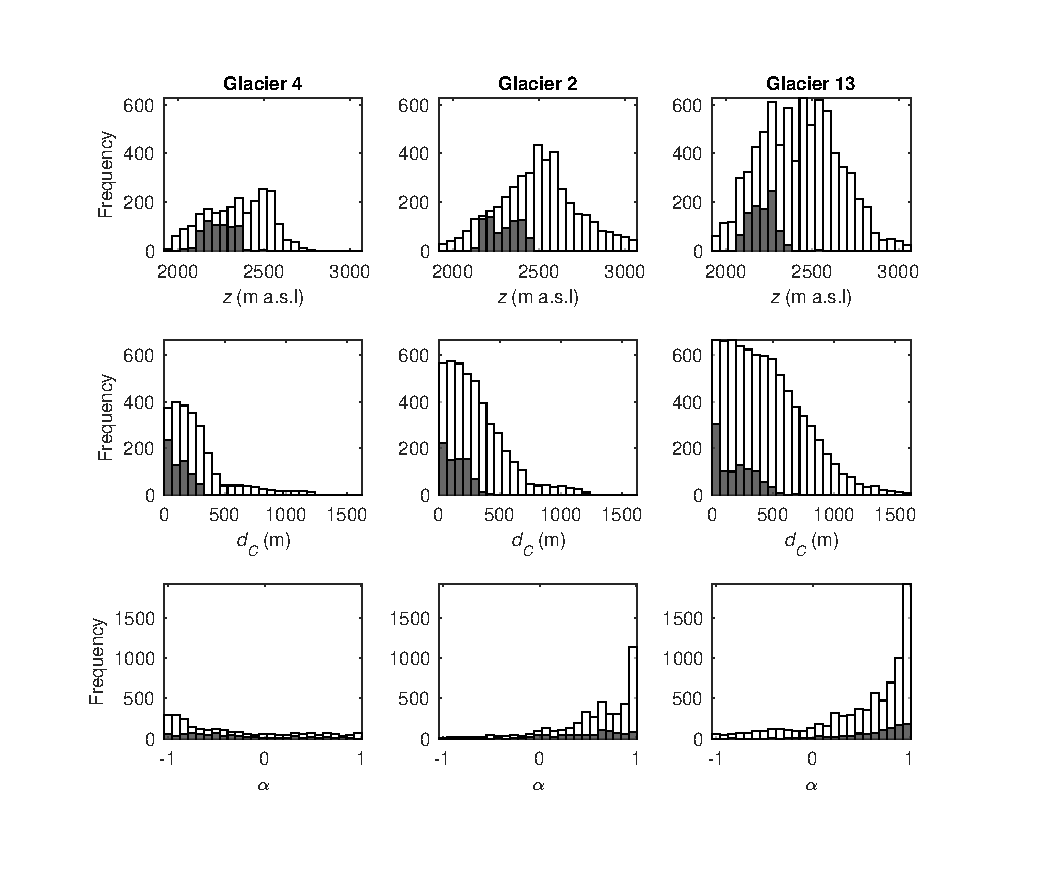
\includegraphics[width =0.9\textwidth]{TopoParamsSampled1.pdf}\\
	\caption{Distribution of sampled (gray bars) and all (white bars) topographic parameters for over Glacier 4 (left column), Glacier 2 (middle column) and Glacier 13 (right column). From top to bottom, topographic parameters are elevation ($z$), distance from centreline ($d_C$), aspect ($\alpha$), slope ($m$), northness ($N$), mean curvature ($\kappa$), and wind redistribution ($Sx$).}
	\label{fig:TopoParamsSampled1}
\end{figure}

\renewcommand{\thefigure}{S\arabic{figure} (Cont.)}
\addtocounter{figure}{-1}

\begin{figure}[]
\centering
	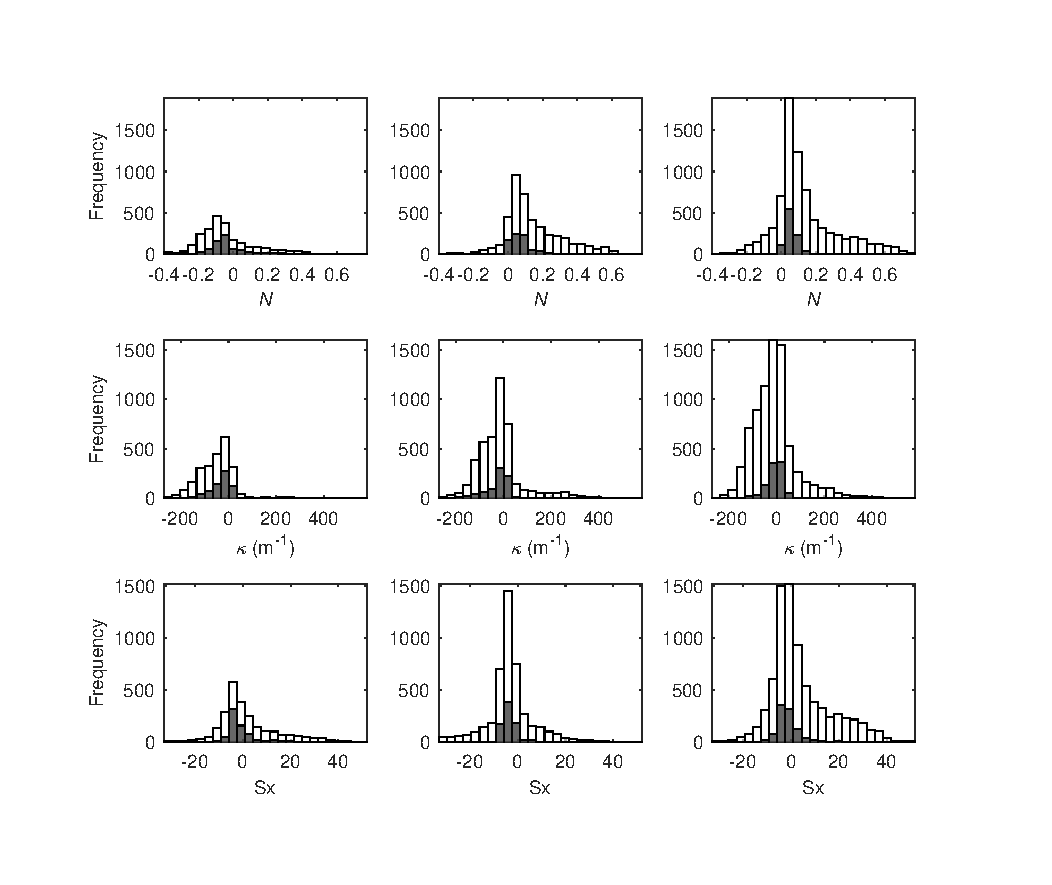
\includegraphics[width =0.9\textwidth]{TopoParamsSampled2.pdf}\\
	\caption{Distribution of sampled (gray bars) and all (white bars) topographic parameters for  Glacier 4 (left column), Glacier 2 (middle column) and Glacier 13 (right column). From top to bottom, topographic parameters are elevation ($z$), distance from centreline ($d_C$), aspect ($\alpha$), slope ($m$), northness ($N$), mean curvature ($\kappa$), and wind redistribution ($Sx$).}
	\label{fig:TopoParamsSampled2}
\end{figure}


%% TOPO PARAMS TABLE
\begin{landscape}
\begin{table}[H]
\begin{threeparttable}
   %\captionsetup{singlelinechec\FloatBarrierk=off, skip=4pt}
\caption{Description of topographic parameters used in the linear regression.}
\label{tab:TopoParams}
\begin{tabularx}{24cm}{XXXXX}

\midrule
\textbf{\begin{tabular}[c]{@{}l@{}}Topographic\\ parameter\end{tabular}} & \textbf{Definition} & \textbf{\begin{tabular}[c]{@{}l@{}}Calculation \\ method\end{tabular}} & \textbf{Notes} & \textbf{Source} \\ \midrule
\textbf{Elevation ($z$)} & Height above mean sea level & Values taken directly from DEM &  &  \\ \midrule
\textbf{Distance from centreline ($d_C$)} & Linear distance from user-defined glacier centreline & Minimum distance between the Easting and Northing of the northwest corner of each grid cell and a manually defined centreline &  &  \\ \midrule
\textbf{Slope ($m$)} & Angle between a plane tangential to the surface (gradient) and the horizontal & \texttt{r.slope.aspect} module in GRASS GIS software run through QGIS &  & \cite{Mitavsova1993, Hofierka2009, Olaya2009} \\ \midrule
\textbf{Aspect ($\alpha$)} & Dip direction of the slope & \texttt{r.slope.aspect} module in GRASS GIS software run through QGIS & $\sin(\alpha)$, a linear quantity describing a slope as north/south facing, is used in the regression & \cite{Mitavsova1993, Hofierka2009, Olaya2009} \\ \midrule
\textbf{Mean curvature ($\kappa$)} & Average of profile (direction of the surface gradient) and tangential (direction of the contour tangent) curvature & \texttt{r.slope.aspect} module in GRASS GIS software run through QGIS & ($+$) mean-concave terrain and ($-$) mean-convex terrain & \cite{Mitavsova1993, Hofierka2009, Olaya2009} \\ \midrule
\textbf{``Northness'' ($N$)} & A value of $-1$ represents a vertical, south facing slope, a value of $+1$ represents a vertical, north facing slope, and a flat surface yields 0 & Product of the cosine of aspect and sine of slope &  & \citep{Molotch2005} \\ \midrule
\textbf{Wind exposure/shelter parameter (Sx)} & Proxy for snow deposition due to wind redistribution & Executable obtained from Adam Winstral that follows the procedure outlined in \cite{Winstral2002} & Calculation based on selecting a cell within a certain angle and distance from the cell of interest that has the greatest upward slope relative to the cell of interest & \citep{Winstral2002}
\end{tabularx}
\end{threeparttable}
\end{table}
\end{landscape}


\clearpage

%%%%%%%%%%%%%%%%%%%%%%%%%%%%%%%%%%%%%%%%%
% Additional Results
%%%%%%%%%%%%%%%%%%%%%%%%%%%%%%%%%%%%%%%%%

\subsection*{Additional results}

%% DENSITY VALUES USED
\begin{table}[h]
\centering
\caption{Snow density values used for density assignment methods. Density values derived from snow pit (SP) densities and Federal Sampler (FS) densities. Four interpolation methods are chosen: (1) using a mean snow density for all three glaciers (S1 or F1), (2) using a mean density for each glacier (S2 or F2), (3) using a regression between density and elevation (S3 or F3), and (4) inverse-distance weighted mean density (not shown, S4 or F4). Standard deviation (STD) is given for S1/F1 and S2/F2 values and R$^2$ values are given for density--elevation regressions (S3/F3).}
\label{tab:Density}
\begin{tabular}{cccccc}
\midrule
\textbf{} &  & \multicolumn{2}{c}{\textbf{\begin{tabular}[c]{@{}c@{}}SP-derived\\ density (kg\,m$^{-3}$)\end{tabular}}} & \multicolumn{2}{c}{\textbf{\begin{tabular}[c]{@{}c@{}}FS-derived\\ density (kg\,m$^{-3}$)\end{tabular}}} \\
\textbf{} &  & \textit{Mean} & \textit{STD or R$^2$} & \textit{Mean} & \textit{STD or R$^2$} \\ \midrule
\textbf{S1 or F1} &  & 342 & 26 & 318 & 42 \\ \midrule
\multirow{3}{*}{\textbf{S2 or F2}} & G4 & 348 & 13 & 355 & 18 \\
 & G2 & 333 & 26 & 286 & 34 \\
 & G13 & 349 & 38 & 316 & 41 \\ \midrule
\multirow{3}{*}{\textbf{S3 or F3}} & G4 & $0.03z+274$ & 0.16 & $-0.16z+714$ & 0.53 \\
 & G2 & $-0.14z+659$ & 0.75 & $0.24z-282$ & 0.72 \\
 & G13 & $-0.20z+802$ & $>$0.99 & $0.12z+33$ & 0.21
\end{tabular}
\end{table}



\renewcommand{\thefigure}{S\arabic{figure}}
\addtocounter{figure}{+1}

%% Gridcell-averaged $B_\mathrm{w}$ values
\begin{figure}[H]
\centering
	\includegraphics[width =0.5\textwidth]{GridcellWB_boxplot.png}\\
	\caption{Boxplot of gridcell-averaged winter balance on three study glaciers. \boxMatlab}
	\label{fig:GridcellWB_boxplot}
\end{figure}

%% Standard deviation of point-scale $B_\mathrm{w}$ values within a gridcell measured along transects
\begin{figure}[H]
\centering
	\includegraphics[width = 0.8\textwidth]{DEMcellSTD.png}\\
	\caption[]{Boxplot of the standard deviation of measured winter balance in one DEM gridcell. \boxMatlab}
	\label{fig:DEMcellSTD}
\end{figure}


%% Standard deviation maps
\pagebreak
\begin{figure}[H]
	\centering
	\includegraphics[width =0.8\textwidth]{LRstd_map_gridcell.pdf}\\
	\includegraphics[width =0.8\textwidth]{LRstd_map_density.pdf}\\
	\includegraphics[width =0.8\textwidth]{LRstd_map_int.pdf}\\
	\caption{Standard deviation (STD) of distributed winter balance ($b_\mathrm{w}$) arising from (top row) gridcell-scale variability, (middle row) method of density assignment and (bottom row) interpolation uncertainty found using linear regression. Ice-flow directions are indicated by arrows.}
\end{figure}

\begin{figure}[H]
	\centering
	\includegraphics[width =0.8\textwidth]{OKstd_map_gridcell.pdf}\\
	\includegraphics[width =0.8\textwidth]{OKstd_map_density.pdf}\\
	\includegraphics[width =0.8\textwidth]{OKstd_map_int.pdf}\\
	\caption{Standard deviation (STD) of distributed winter balance ($b_\mathrm{w}$) arising from (top row) gridcell-scale variability, (middle row) method of density assignment and (bottom row) interpolation uncertainty found using ordinary kriging. Ice-flow directions are indicated by arrows.}
\end{figure}

\vfill

%% RK

\section{Regression kriging}
\label{sec:regressionkriging}

\subsection{Background}

Regression kriging (RK) estimates values between measurement locations by combining a regression estimate with a kriged estimate of the regression residuals \citep{Hengl2007}. First, the regression estimate is determined using auxiliary variables (e.g. topographic parameters). Then, OK is used to interpolate regression residuals, which have an assumed mean of zero. The two surface estimates are then added. The final estimate can be written as 
\begin{align}
\hat{z}(x_0) &= \hat{m}(x_0) + \hat{e}(x_0)\\
& = \sum^p_{k=0}\hat{\beta}_k \cdot	q_k(x_0)+ \sum_{i=1}^{n} \lambda_i \cdot e(x_i),
\end{align}
where $\hat{m}(x_0)$ is the regression estimate and $\hat{e}(x_0)$ is the interpolated residual, $\hat{\beta}_k$ are the estimated regression coefficients, $q_k(x_0)$ are the regressors, $p$ is the number of regressors, $\lambda_i$ are the kriging weights for the residuals and $e(x_i)$ is the residual at $x_i$. 

RK can be thought of as an intermediate between pure kriging (no auxiliary variables) and pure regression (small residuals) and can be more strongly skewed to either end-member based on the strength of the regression correlation \citep{Hengl2007}. RK is mathematically equivalent to universal kriging, in which auxiliary variables are used directly to determine the kriging weights \citep{Hengl2007}. However, separating the trend analysis and kriging steps has the advantage of being able to test interpolation methods that go beyond a basic linear trend. Kriging combined with regression has been found to produce better estimates of spatial fields when compared to OK and co-kriging \citep[e.g.][]{Knotters1995}.

\subsection{Methods}

Distributed $b_\mathrm{w}$ values are first estimated with a LR of gridcell-averaged $b_\mathrm{w}$ on topographic parameters, as described in the manuscript. Second, the residuals at each measurement location are calculated and the distributed residuals are found using OK, as described above. The LR and OK-estimated residuals are then added together to obtain the final distributed $b_\mathrm{w}$. 

\subsection{Results}

The range of residual values is highest on Glacier 4 and lowest on Glacier 13 (Figure \ref{fig:residualsKRIGING}). Extreme values are located in the accumulation area of Glacier 4 with both strongly negative and strongly positive residuals located within a kilometre of each other. The low sampling density in the accumulation area biases the interpolation of residuals to fit the over- and under-estimated values of $B_\mathrm{w}$ at the two uppermost sampling locations. Residuals show less variation on Glacier 2, although relatively large residuals of approximately $\pm 0.4$ \,m\,w.e. are present in the upper ablation area along the ice margins. Glacier 13 has the smallest range of residuals. The glacier-wide value of distributed residuals is positive for Glacier 4, indicating that the distributed residuals will increase the overall estimate of $B_\mathrm{w}$. Conversely, the glacier-wide residual for Glacier 2 is negative and will decrease the estimated $B_\mathrm{w}$. 

Spatial patterns in estimated $B_\mathrm{w}$ found using RK are similar to those found with both OK and regression (Figure \ref{fig:Regression-Kriging}) for Glaciers 2 and 13. The RK estimate is closer to the linear regression for Glaciers 2 and 13 due to the relatively high explanatory power of the regressions for these glaciers. The distributed $B_\mathrm{w}$ on Glacier 4 found using RK is somewhat uniform in the central region of the glacier, but the accumulation area has considerably larger estimates of $B_\mathrm{w}$ compared to OK and regression. The spatial patterns of distributed $B_\mathrm{w}$ on Glacier 4 more strongly resemble those of the distributed residuals (Figure \ref{fig:residualsKRIGING}). This supports the idea that $B_\mathrm{w}$ estimates are more strongly affected by the kriged residuals because the regression had low explanatory power. RK applied to Glacier 4 is therefore closer to OK. The marked alteration of the regression estimate by the kriged residuals arises from the large and opposing residual values at the upper-most measurement locations. Higher $B_\mathrm{w}$ values in the accumulation area result in a much higher estimate of glacier-wide $B_\mathrm{w}$. The large effect of two measurement locations on the glacier-wide $B_\mathrm{w}$ highlights the over representation of individual data points in under-sampled regions.

Both OK and RK produce a gradient in glacier-wide $B_\mathrm{w}$ across the mountain range (Figure \ref{fig:Regression-Kriging}). Glacier 4 has the highest glacier-wide $B_\mathrm{w}$ and Glacier 13 has the lowest glacier-wide $B_\mathrm{w}$. However, the $B_\mathrm{w}$ gradient is steeper for OK estimates when compared with RK estimates. Glacier 4 has a similar glacier-wide $B_\mathrm{w}$ between the two methods but glacier-wide $B_\mathrm{w}$ on Glaciers 2 and 13 are much lower than on Glacier 4.  

RK produces the highest overall set of R$^2$ values (Figure \ref{fig:R2regressionkrig}). The correlation coefficient for Glacier 2 is especially high, with more than 80\% of the observed variance explained by the RK model. Glacier 4 has the lowest correlation coefficient but this value is considerably higher than that arising from topographic regression or OK alone. 

\begin{figure}
	\centering
	\includegraphics[width = 0.7\textwidth]{residualsKriged.png}\\
	\caption[Distributed Bayesian model averaging residuals estimated by regression kriging (RK)]{Distributed Bayesian model averaging residuals estimated by regression kriging (RK). \topomap Dashed line indicates approximate ELA.}
	\label{fig:residualsKRIGING}
\end{figure}

\begin{figure}
	\centering
	\includegraphics[width = 0.7\textwidth]{RegressionKriging.png}\\
	\caption[Winter balance estimated by adding kriged regression residuals to winter balance estimated using topographic regression with Bayesian model averaging]{Winter balance estimated by adding kriged regression residuals to winter balance estimated using topographic regression with Bayesian model averaging. \swedots}
	\label{fig:Regression-Kriging}
\end{figure}

\begin{figure}
	\makebox[\textwidth][c]{\includegraphics[width=0.8\textwidth]{krigRKfit.png}}%
	\caption[Comparison of estimated (regression kriging, RK) and observed winter balance ($B_\mathrm{w}$) for study glaciers]{Comparison of estimated (regression kriging, RK) and observed winter balance ($B_\mathrm{w}$) for study glaciers. The $B_\mathrm{w}$ values are calculated using inverse-distance weighted snow-pit densities (S4).}
	\label{fig:R2regressionkrig}
\end{figure}




%----------------------------------------------------------------------------------------
%	REFERENCE LIST
%----------------------------------------------------------------------------------------
\clearpage
%\bibliography{/home/glaciology1/Documents/MastersDocuments/MastersLit}
\bibliography{/Users/Alexandra/Documents/SFU/MastersDocuments/MastersLit}
\bibliographystyle{igs}

%----------------------------------------------------------------------------------------


\end{document}